\documentclass[UTF8,fontset=none,aspectratio=169,10pt]{beamer}
\usepackage{ads-beamer-theme}

\title{高级分布式系统}
\subtitle{第三讲：逻辑时间与物理时钟同步}
\author{陈鹏飞\quad 计算机学院}
\institute{中山大学}
\date{2025--2026 学年}

\begin{document}

\begin{frame}[plain]
\begin{tikzpicture}[remember picture,overlay]
  \fill[ADSBlue] (current page.north west) rectangle ([xshift=2.4cm]current page.south west);
  \fill[ADSOrange] ([xshift=2.4cm]current page.north west) rectangle ([xshift=2.55cm]current page.south west);
  \node[anchor=west,align=left] at ([xshift=3.3cm,yshift=1.0cm]current page.west) {\fontsize{32}{38}\selectfont\color{ADSBlue}\bfseries 高级分布式系统};
  \node[anchor=west,align=left] at ([xshift=3.3cm,yshift=-0.4cm]current page.west) {\fontsize{21}{27}\selectfont\color{ADSDarkBlue}第三讲\quad 逻辑时间与物理时钟同步};
  \node[anchor=west,align=left] at ([xshift=3.3cm,yshift=-2.2cm]current page.west) {\large\color{ADSGray}没有全局时钟，仍然可以表达因果、知识与系统进度};
  \node[anchor=east] at ([xshift=-0.8cm,yshift=-3.2cm]current page.east) {\small\color{ADSGray}陈鹏飞\quad 中山大学\quad 2025--2026};
  \draw[ADSBlue,line width=0.8pt] ([xshift=3.3cm,yshift=-1.35cm]current page.west) -- ([xshift=12.6cm,yshift=-1.35cm]current page.west);
\end{tikzpicture}
\end{frame}

\begin{frame}{本讲学习目标}
\begin{enumerate}
  \item 解释逻辑时钟的时间域、时间戳和一致性条件；
  \item 正确执行 Lamport 标量时钟与向量时钟更新算法；
  \item 用时间戳判断因果、并发和事件高度；
  \item 理解差分向量时钟与矩阵时钟的语义和代价；
  \item 解释 Virtual Time、Time Warp、反消息与回滚；
  \item 推导 NTP 的 offset、delay，并理解物理时钟误差。
\end{enumerate}
\vfill
\callout{核心能力}{知道一个时间戳“能证明什么、不能证明什么”，比会套公式更重要。}
\end{frame}

\begin{frame}{本讲结构}
\begin{columns}[T,onlytextwidth]
\column{.18\textwidth}\callout{Part I}{逻辑时钟框架}
\column{.18\textwidth}\callout{Part II}{标量与向量时间}
\column{.18\textwidth}\callout{Part III}{差分与矩阵时间}
\column{.18\textwidth}\callout{Part IV}{Virtual Time}
\column{.18\textwidth}\callout{Part V}{NTP 物理同步}
\end{columns}
\vfill
\begin{center}
\begin{tikzpicture}[node distance=7mm]
\nodebox{ADSBlue}{cause}{因果};
\nodebox[right=of cause]{ADSOrange}{stamp}{时间戳};
\nodebox[right=of stamp]{ADSGreen}{knowledge}{知识};
\nodebox[right=of knowledge]{ADSGray}{sync}{同步};
\draw[ADSBlue,\arrow] (cause)--(stamp);
\draw[ADSOrange,\arrow] (stamp)--(knowledge);
\draw[ADSGreen,\arrow] (knowledge)--(sync);
\end{tikzpicture}
\end{center}
\end{frame}

\sectionframe{逻辑时钟的统一框架}{逻辑时间不是模拟墙上时钟，而是把因果偏序编码为可比较的数据结构。}

\begin{frame}{为什么分布式系统首先需要“逻辑时间”}
\begin{itemize}
  \item 因果关系是并行与分布式系统设计、分析和调试的基础；
  \item 集中式系统常用一个物理时钟描述“先后”；
  \item 分布式系统没有可瞬时读取的全局物理时钟；
  \item 异步计算的进展呈突发性，墙上时间相近并不代表存在因果；
  \item 对许多算法，保持因果单调性已经足够。
\end{itemize}
\vfill
\callout{关键区分}{物理时间回答“现实世界大约几点”；逻辑时间回答“哪些事件必须先于哪些事件”。}
\end{frame}

\begin{frame}{因果关系比“时间接近”更稳定}
\begin{columns}[T,onlytextwidth]
\column{.47\textwidth}
\blocktitle{物理时间可能误导}
\begin{itemize}
  \item 时钟有 offset 与 skew；
  \item 网络延迟不对称；
  \item 同一事件在不同日志中时间戳不同；
  \item NTP 调整可能造成时间跳变。
\end{itemize}
\column{.47\textwidth}
\blocktitle{因果关系依赖证据}
\begin{itemize}
  \item 同一进程的程序顺序；
  \item 消息发送先于对应接收；
  \item 关系的传递闭包；
  \item 与具体秒数无关。
\end{itemize}
\end{columns}
\vfill
\callout{工程含义}{Trace、版本向量和复制协议通常关心因果，而监控告警和审计还需要物理时间。}
\end{frame}

\begin{frame}{三种逻辑时间：标量、向量与矩阵}
\begin{tabularx}{\linewidth}{>{\bfseries}p{2.4cm}XXX}
\toprule
系统 & 数据结构 & 可表达信息 & 主要代价 \\
\midrule
标量时间 & 一个整数 & 因果蕴含数值先后；可构造全序 & 丢失并发信息 \\
向量时间 & $n$ 维向量 & 精确表达因果与并发 & 消息和状态开销 $O(n)$ \\
矩阵时间 & $n\times n$ 矩阵 & “我知道别人知道什么” & 开销可达 $O(n^2)$ \\
\bottomrule
\end{tabularx}
\vfill
\callout{共同目标}{都要保证：事件沿因果路径前进时，时间戳严格单调。}
\end{frame}

\begin{frame}{逻辑时钟系统的形式化定义}
逻辑时钟系统由时间域 $T$ 与映射 $C$ 组成：
\[
C:H\rightarrow T,
\]
其中 $H$ 是分布式执行中的事件集合，$T$ 在关系 $<$ 下构成偏序集。
\vfill
事件 $e$ 的时间戳为 $C(e)$。时钟必须满足：
\[
e_i\rightarrow e_j\quad\Longrightarrow\quad C(e_i)<C(e_j).
\]
\vfill
\callout{含义}{逻辑时钟必须尊重因果，但不同系统对“反方向是否成立”的能力不同。}
\end{frame}

\begin{frame}{Clock consistency：因果一定导致时间前进}
\begin{center}
\begin{tikzpicture}[node distance=15mm]
\nodebox{ADSBlue}{e}{事件 $e_i$};
\nodebox[right=of e]{ADSOrange}{f}{事件 $e_j$};
\draw[ADSBlue,\arrow] (e)--node[above]{因果路径} (f);
\node[below=11mm of e,draw=ADSBlue,rounded corners,fill=ADSBlue!6,minimum width=2.2cm,minimum height=.8cm] {$C(e_i)$};
\node[below=11mm of f,draw=ADSOrange,rounded corners,fill=ADSOrange!8,minimum width=2.2cm,minimum height=.8cm] {$C(e_j)$};
\draw[ADSOrange,\arrow] ([yshift=-11mm]e.south)--node[below]{$<$} ([yshift=-11mm]f.south);
\end{tikzpicture}
\end{center}
\vfill
\begin{itemize}
  \item 该单调性称为时钟一致性条件；
  \item 若算法违反它，时间戳会把结果排在原因之前；
  \item 一致性只给出充分证据：$e_i\rightarrow e_j$ 足以推出时间先后。
\end{itemize}
\end{frame}

\begin{frame}{Strong consistency：时间比较等价于因果比较}
强一致逻辑时钟满足双向条件：
\[
e_i\rightarrow e_j
\quad\Longleftrightarrow\quad
C(e_i)<C(e_j).
\]
\vfill
\begin{columns}[T,onlytextwidth]
\column{.47\textwidth}
\blocktitle{一致但不强一致}
\begin{itemize}
  \item 因果事件一定递增；
  \item 递增时间戳未必表示因果；
  \item Lamport 标量时钟属于此类。
\end{itemize}
\column{.47\textwidth}
\blocktitle{强一致}
\begin{itemize}
  \item 时间戳完整保留偏序；
  \item 可直接判断因果与并发；
  \item 标准向量时钟属于此类。
\end{itemize}
\end{columns}
\end{frame}

\begin{frame}{实现框架：局部逻辑时钟与全局视图}
每个进程 $p_i$ 维护两类能力：
\begin{itemize}
  \item 局部逻辑时钟 $lc_i$：度量自身进展；
  \item 逻辑全局时钟 $gc_i$：表示 $p_i$ 对全局逻辑时间的局部视图；
  \item 通常 $lc_i$ 是 $gc_i$ 的一个组成部分；
  \item 每个进程只有局部视图，不存在一个被所有节点瞬时共享的变量。
\end{itemize}
\vfill
\callout{知识解释}{$gc_i$ 不是“真实全局状态”，而是进程 $p_i$ 通过本地执行和收到的消息积累的知识。}
\end{frame}

\begin{frame}{通用更新协议：R1 与 R2}
\begin{columns}[T,onlytextwidth]
\column{.47\textwidth}
\blocktitle{R1：本地事件规则}
\begin{itemize}
  \item 在执行 internal、send 或 receive 事件时更新本地逻辑时间；
  \item 确保同一进程上的事件严格递增；
  \item 描述进程自身的进展。
\end{itemize}
\column{.47\textwidth}
\blocktitle{R2：消息合并规则}
\begin{itemize}
  \item 发送方在消息中携带时间信息；
  \item 接收方把远端知识合并到本地全局视图；
  \item 再执行 R1，保证接收晚于发送。
\end{itemize}
\end{columns}
\vfill
\callout{系统差异}{标量、向量和矩阵时钟的主要差别，正是时间结构以及 R1/R2 的具体定义。}
\end{frame}

\begin{frame}{一个时间戳系统需要回答四个问题}
\begin{enumerate}
  \item \key{表示：}时间域是整数、向量、矩阵，还是其他结构？
  \item \key{更新：}本地事件与消息接收如何改变时间？
  \item \key{比较：}两个时间戳的 $<$、$=$、并发如何定义？
  \item \key{语义：}比较结果能证明因果、并发、知识还是物理先后？
\end{enumerate}
\vfill
\begin{center}
\begin{tikzpicture}[node distance=7mm]
\nodebox{ADSBlue}{rep}{表示};
\nodebox[right=of rep]{ADSOrange}{update}{更新};
\nodebox[right=of update]{ADSGreen}{compare}{比较};
\nodebox[right=of compare]{ADSGray}{meaning}{语义};
\draw[ADSBlue,\arrow] (rep)--(update);
\draw[ADSOrange,\arrow] (update)--(compare);
\draw[ADSGreen,\arrow] (compare)--(meaning);
\end{tikzpicture}
\end{center}
\end{frame}

\sectionframe{Lamport 标量时间}{用一个整数保持因果单调，并通过进程编号把偏序扩展为全序。}

\begin{frame}{标量时间：把局部与全局视图压缩为一个整数}
Lamport 于 1978 年提出标量逻辑时钟。对进程 $p_i$：
\begin{itemize}
  \item 时间域为非负整数；
  \item 用单个变量 $C_i$ 同时表示局部进展和对全局时间的视图；
  \item 目标是让 happened-before 蕴含时间戳递增；
  \item 单个整数无法保存“我分别知道各进程进展到哪里”。
\end{itemize}
\vfill
\callout{设计选择}{压缩带来常数级开销，也必然丢失因果依赖的结构信息。}
\end{frame}

\begin{frame}{标量时钟 R1：执行事件前递增}
在执行任意 internal、send 或 receive 事件之前：
\[
C_i:=C_i+d,\qquad d>0.
\]
通常取 $d=1$。
\vfill
\begin{itemize}
  \item 本地事件的时间戳严格递增；
  \item 不同事件可使用不同正增量，但会影响“事件计数”语义；
  \item 发送事件的消息携带更新后的 $C_i$。
\end{itemize}
\end{frame}

\begin{frame}{标量时钟 R2：接收时合并发送方时间}
消息 $m$ 携带发送时的时间戳 $C_{msg}$。进程 $p_i$ 收到消息后：
\begin{enumerate}
  \item $C_i:=\max(C_i,C_{msg})$；
  \item 执行 R1，即 $C_i:=C_i+d$；
  \item 以新的 $C_i$ 为接收事件时间戳并交付消息。
\end{enumerate}
因此在 $d=1$ 时可合并写为：
\[
C_i:=\max(C_i,C_{msg})+1.
\]
\vfill
\callout{因果保证}{接收事件的时间戳严格大于对应发送事件。}
\end{frame}

\begin{frame}{标量时间的演化示例}
\begin{center}
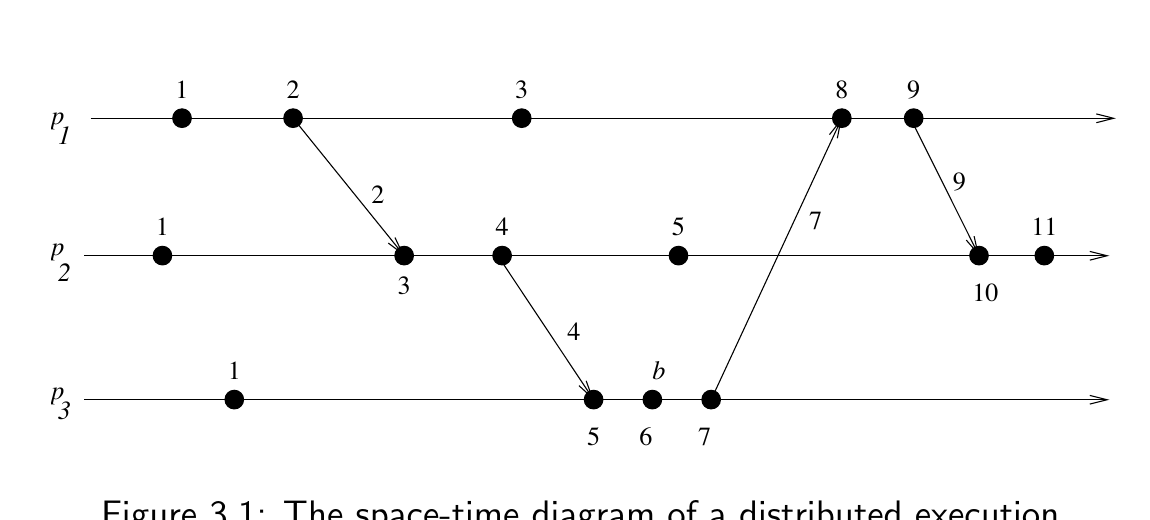
\includegraphics[trim=0 58 0 0,clip,width=.93\linewidth,height=.60\paperheight,keepaspectratio]{assets/week03-source-2025/scalar-time-evolution.png}
\end{center}
\smallnote{图示：进程内按 R1 递增，消息接收按 $\max$ 合并后再递增。}
\end{frame}

\begin{frame}{沿图计算：每次接收都做一次“最大值 + 1”}
\begin{columns}[T,onlytextwidth]
\column{.44\textwidth}
\begin{enumerate}
  \item $p_1$ 在时间 2 发送；
  \item $p_2$ 原值为 1，接收后变为 $\max(1,2)+1=3$；
  \item $p_2$ 在时间 4 发送；
  \item $p_3$ 接收后变为 $\max(1,4)+1=5$。
\end{enumerate}
\column{.51\textwidth}
\begin{center}
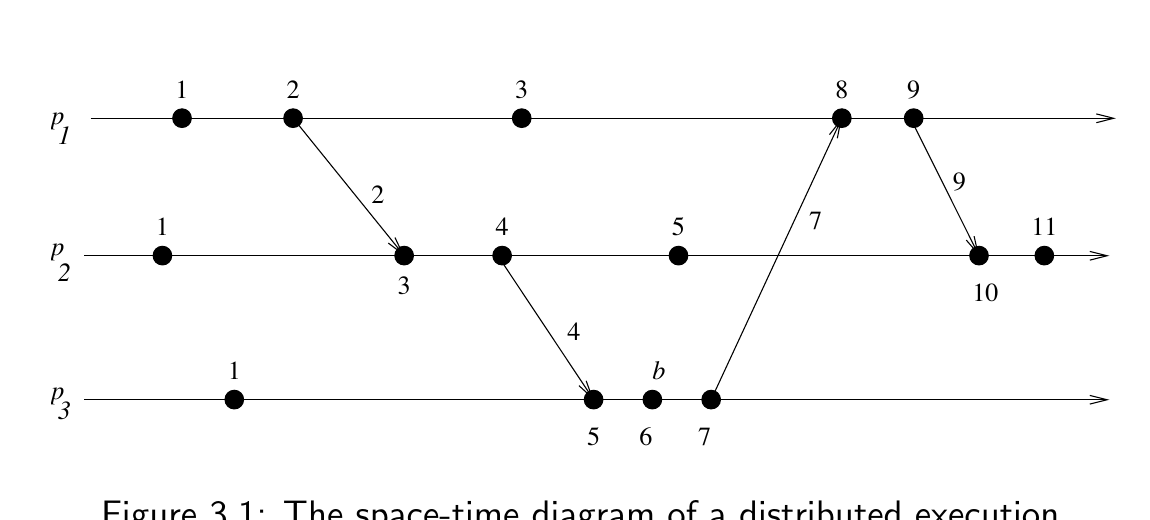
\includegraphics[trim=0 58 0 0,clip,width=\linewidth,height=.47\paperheight,keepaspectratio]{assets/week03-source-2025/scalar-time-evolution.png}
\end{center}
\end{columns}
\vfill
\callout{检查方法}{沿任意进程线和消息箭头向右走，标量时间必须严格增加。}
\end{frame}

\begin{frame}{基本性质：标量时钟满足一致性}
对任意两个事件 $e_i,e_j$：
\[
e_i\rightarrow e_j\quad\Longrightarrow\quad C(e_i)<C(e_j).
\]
证明只需检查 happened-before 的生成规则：
\begin{itemize}
  \item 同一进程顺序由 R1 保证；
  \item 发送到接收由 R2 保证；
  \item 传递闭包由整数 $<$ 的传递性保证。
\end{itemize}
\vfill
\callout{证明套路}{先对因果关系的基本边证明，再利用传递性扩展到任意因果路径。}
\end{frame}

\begin{frame}{仅靠整数时间戳不能直接得到全序}
不同进程上的事件可能获得相同标量时间戳：
\[
C(e)=C(f),\qquad e\neq f.
\]
\begin{itemize}
  \item 相同时间戳并不表示同一事件；
  \item 也不表示事件在物理世界同时发生；
  \item 若应用需要确定性全序，还必须加入破同值规则；
  \item 多个跨进程事件可能具有相同标量值。
\end{itemize}
\end{frame}

\begin{frame}{用进程编号打破平局：从偏序扩展为全序}
令事件 $x,y$ 的时间戳分别为 $(h,i)$ 与 $(k,j)$，其中第二项是进程编号：
\[
x\prec y
\quad\Longleftrightarrow\quad
h<k\ \lor\ (h=k\land i<j).
\]
\begin{itemize}
  \item 先按标量时间排序；
  \item 时间相同时按预先确定的进程编号排序；
  \item 该关系是确定的全序，并保持 happened-before；
  \item 常用于分布式互斥中的请求排序。
\end{itemize}
\end{frame}

\begin{frame}{全序不等于因果：平局规则只是一种确定性选择}
\begin{center}
\begin{tikzpicture}[node distance=9mm]
\nodebox{ADSBlue}{partial}{因果偏序};
\nodebox[right=of partial]{ADSOrange}{tie}{加入进程编号};
\nodebox[right=of tie]{ADSGreen}{total}{确定性全序};
\draw[ADSBlue,\arrow] (partial)--(tie);
\draw[ADSOrange,\arrow] (tie)--(total);
\end{tikzpicture}
\end{center}
\vfill
\begin{itemize}
  \item 对并发事件，$x\prec y$ 只是算法人为选择的顺序；
  \item 不能从 $x\prec y$ 推断 $x\rightarrow y$；
  \item 全序适合复制日志、仲裁和互斥，但会隐藏真实并发；
  \item 若需要并发信息，应使用向量时间或显式依赖图。
\end{itemize}
\end{frame}

\begin{frame}{事件计数与事件高度}
当所有增量 $d=1$ 且初值为 0 时，若 $C(e)=h$：
\begin{itemize}
  \item $h-1$ 表示产生 $e$ 前至少需要经历的逻辑步骤数；
  \item 它等于以 $e$ 为终点的最长因果链长度（不计 $e$）；
  \item 因此可把 $h$ 看作事件在因果 DAG 中的“高度”；
  \item 教材示例中，事件 $b$ 的时间戳为 6，其最长因果前缀含 5 个事件。
\end{itemize}
\vfill
\callout{限制}{若使用不同的 $d$，时间戳仍保持因果单调，但不再具有直接的事件计数含义。}
\end{frame}

\begin{frame}{标量时间不满足强一致性}
标量时钟只能保证：
\[
e_i\rightarrow e_j\Rightarrow C(e_i)<C(e_j),
\]
但反向不成立：
\[
C(e_i)<C(e_j)\not\Rightarrow e_i\rightarrow e_j.
\]
\begin{itemize}
  \item 两个并发事件也会被整数大小排出先后；
  \item 接收方通过 $\max$ 只记住一个聚合值；
  \item 它忘记这个值分别来自哪些进程、哪些事件；
  \item 因此无法仅凭标量时间判断并发。
\end{itemize}
\end{frame}

\begin{frame}{反例：时间戳更小的事件未必是原因}
\begin{center}
\begin{tikzpicture}[x=1.15cm,y=1.0cm,>=Stealth]
\draw[->,ADSGray] (0,2)--(8,2) node[right]{$p_1$};
\draw[->,ADSGray] (0,0)--(8,0) node[right]{$p_2$};
\fill[ADSBlue] (2,2) circle (2.3pt) node[above]{3};
\fill[ADSOrange] (6,0) circle (2.3pt) node[above]{7};
\node[below=5mm,align=center,text=ADSGray] at (4,1) {两点之间没有消息路径};
\end{tikzpicture}
\end{center}
\vfill
尽管 $3<7$，两个事件仍可能并发。整数顺序只是逻辑时钟的一致扩展，并非因果证据。
\end{frame}

\begin{frame}{课堂互动：给执行图标 Lamport 时间}
\begin{columns}[T,onlytextwidth]
\column{.55\textwidth}
\begin{center}
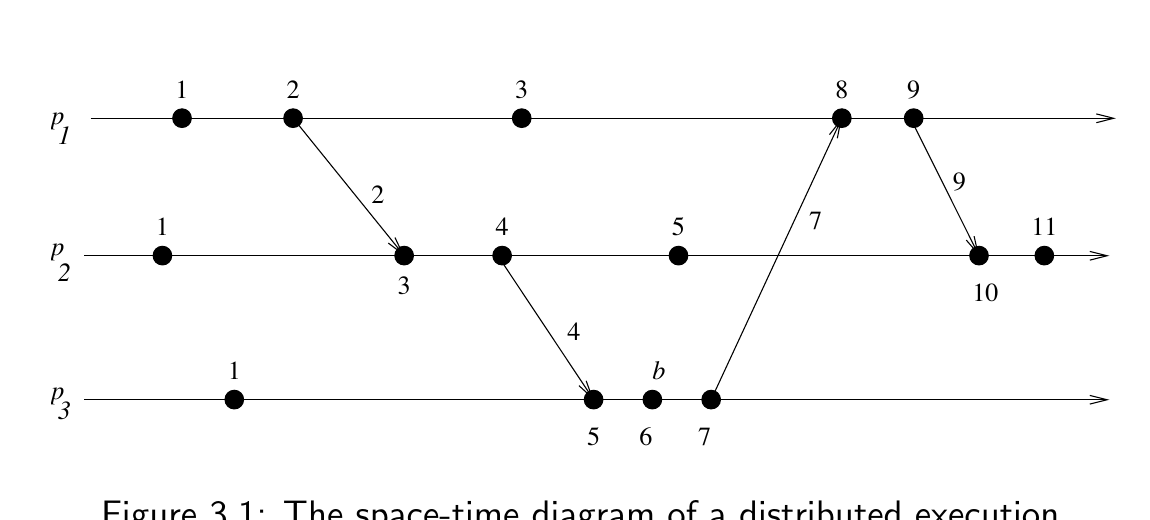
\includegraphics[trim=0 58 0 0,clip,width=\linewidth,height=.50\paperheight,keepaspectratio]{assets/week03-source-2025/scalar-time-evolution.png}
\end{center}
\column{.40\textwidth}
\begin{enumerate}
  \item 擦除图中的数字；
  \item 设所有时钟初值为 0；
  \item 按 $d=1$ 重新标注；
  \item 找出所有同值事件；
  \item 给出一个时间戳递增但不因果的事件对。
\end{enumerate}
\end{columns}
\end{frame}

\sectionframe{向量时间}{让每个进程分别记录对所有进程的最新知识，从而保留因果偏序。}

\begin{frame}{向量时钟：每个分量对应一个进程的进展}
向量时钟由 Fidge、Mattern 和 Schmuck 分别提出。进程 $p_i$ 维护：
\[
VT_i[1..n].
\]
\begin{itemize}
  \item $VT_i[i]$ 是 $p_i$ 的局部逻辑时钟；
  \item $VT_i[j]$ 是 $p_i$ 已知的 $p_j$ 最新逻辑时间；
  \item 整个向量构成 $p_i$ 对全局逻辑时间的局部视图；
  \item 事件时间戳是事件发生时该进程的向量值。
\end{itemize}
\end{frame}

\begin{frame}{知识语义：$VT_i[j]=x$ 究竟表示什么}
\begin{center}
\Large
$VT_i[j]=x$
\end{center}
表示进程 $p_i$ 已经获得证据：进程 $p_j$ 的本地逻辑时间至少进展到 $x$。
\vfill
\begin{itemize}
  \item 这个知识通过消息沿因果路径传播；
  \item 若 $p_i$ 尚未收到相关信息，其分量可能落后；
  \item 向量时间描述“我知道的进展”，不是所有节点的瞬时真实状态；
  \item 每个分量保留来源，因此不会像标量 $\max$ 那样完全压平依赖。
\end{itemize}
\end{frame}

\begin{frame}{向量时钟 R1：只递增自己的分量}
在执行任意事件之前，进程 $p_i$ 更新：
\[
VT_i[i]:=VT_i[i]+d,qquad d>0.
\]
通常取 $d=1$。
\begin{itemize}
  \item 本地事件只直接改变第 $i$ 个分量；
  \item 其他分量只能通过收到消息而增长；
  \item 因此每个分量具有清晰的来源与知识含义。
\end{itemize}
\end{frame}

\begin{frame}{向量时钟 R2：逐分量取最大值}
消息 $m$ 携带发送方向量 $VT$。进程 $p_i$ 接收 $(m,VT)$ 后：
\[
\forall k\in[1,n],\qquad VT_i[k]:=\max(VT_i[k],VT[k]),
\]
然后执行 R1 并交付消息。
\vfill
\begin{itemize}
  \item 逐分量 $\max$ 合并双方已知的因果历史；
  \item 再递增自己的分量，记录新的接收事件；
  \item 向量初始值通常为 $[0,0,\ldots,0]$。
\end{itemize}
\end{frame}

\begin{frame}{向量时间的演化示例}
\begin{center}
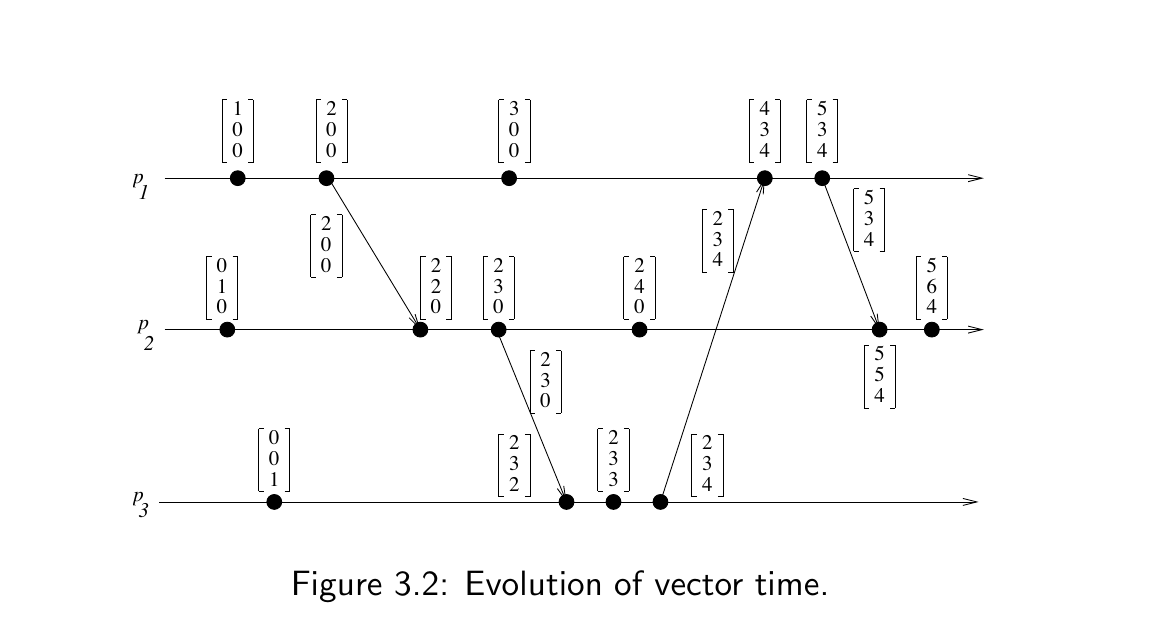
\includegraphics[trim=0 62 0 0,clip,width=.94\linewidth,height=.61\paperheight,keepaspectratio]{assets/week03-source-2025/vector-time-evolution.png}
\end{center}
\smallnote{图示：每个点旁的列向量表示该事件的向量时间戳。}
\end{frame}

\begin{frame}{手算一次消息接收}
假设 $p_2$ 当前向量为 $[2,3,0]$，收到 $p_3$ 携带的 $[2,2,4]$：
\[
\max([2,3,0],[2,2,4])=[2,3,4].
\]
随后 $p_2$ 执行接收事件并递增自己的分量：
\[
VT_2=[2,4,4].
\]
\vfill
\callout{读法}{$p_2$ 知道 $p_1$ 至少发生 2 个事件、自己发生 4 个事件、$p_3$ 至少发生 4 个事件。}
\end{frame}

\begin{frame}{比较两个向量时间戳}
对向量 $V$ 与 $W$ 定义：
\[
\begin{aligned}
V=W &\iff \forall k,\ V[k]=W[k],\\
V\le W &\iff \forall k,\ V[k]\le W[k],\\
V<W &\iff V\le W\ \land\ \exists k,\ V[k]<W[k].
\end{aligned}
\]
若既非 $V<W$ 也非 $W<V$，则二者不可比，记为：
\[
V\parallel W.
\]
\end{frame}

\begin{frame}{向量时间与因果偏序同构}
若事件 $x,y$ 的向量时间戳分别为 $V_x,V_y$，则：
\[
x\rightarrow y
\quad\Longleftrightarrow\quad
V_x<V_y.
\]
并且：
\[
x\parallel y
\quad\Longleftrightarrow\quad
V_x\parallel V_y.
\]
\vfill
\callout{强一致性}{标准向量时钟完整保留事件偏序：比较向量即可判断因果或并发。}
\end{frame}

\begin{frame}{为什么不可比正好表示并发}
考虑：
\[
V=[3,1,0],\qquad W=[2,2,0].
\]
\begin{itemize}
  \item 第一分量 $V[1]>W[1]$；
  \item 第二分量 $V[2]<W[2]$；
  \item 因而 $V\nless W$ 且 $W\nless V$；
  \item 两个事件各自包含对方没有的因果历史，故不存在单向因果路径。
\end{itemize}
\vfill
\callout{几何直觉}{向量偏序中的“交叉分量”就是并发的证据。}
\end{frame}

\begin{frame}{已知事件所在进程时，可简化比较}
若事件 $x$ 发生于 $p_i$、事件 $y$ 发生于 $p_j$，时间戳分别为 $V_x,V_y$，\textbf{完整判定仍须比较所有分量}：
\[
x\rightarrow y\quad\Longleftrightarrow\quad
\bigl(\forall k,\ V_x[k]\le V_y[k]\bigr)\ \land\ \bigl(\exists k,\ V_x[k]<V_y[k]\bigr).
\]
已知发生进程时，$V_x[i]\le V_y[i]$ 只是必要条件，不能单独推出因果关系；若存在任意交叉分量（例如 $V_x[i]>V_y[i]$ 且 $V_x[j]<V_y[j]$），可立即判定两事件并发，但这不是所有并发情形的完整判据。
\vfill
\smallnote{使用局部必要条件只能做快速筛选；最终结论必须回到全分量偏序比较。}
\end{frame}

\begin{frame}{向量时钟满足强一致性}
\begin{itemize}
  \item 本地递增保存进程内顺序；
  \item 消息携带完整向量，把发送方的因果历史传播给接收方；
  \item 逐分量最大值等价于合并两个因果过去；
  \item 因此 $V_x<V_y$ 不只是数值现象，而是存在因果路径的充分必要条件。
\end{itemize}
\vfill
\callout{对比标量}{标量时钟只保存“高度”；向量时钟还保存高度由哪些进程贡献。}
\end{frame}

\begin{frame}{向量时钟的事件计数语义}
当 $d=1$ 时：
\begin{itemize}
  \item $VT_i[i]$ 是进程 $p_i$ 已发生的事件数；
  \item 若事件 $e$ 的时间戳为 $V_e$，则 $V_e[j]$ 是 $p_j$ 上因果先于 $e$ 的事件数；
  \item $\sum_j V_e[j]-1$ 是 $e$ 的因果过去中事件总数；
  \item 这比标量高度更丰富：不仅知道最长链，还知道各进程贡献。
\end{itemize}
\end{frame}

\begin{frame}{为什么强一致向量通常需要 $n$ 个分量}
Charron-Bost 的结果表明：一般情况下，若要对任意 $n$ 进程计算完整保持因果偏序，向量维数不能小于 $n$。
\vfill
\begin{itemize}
  \item 每个并发进程都可能贡献独立因果维度；
  \item 少一个维度就可能把两个不同的因果历史压缩为同一表示；
  \item 因此 $O(n)$ 并非简单实现造成的浪费，而是强一致表达能力的代价；
  \item 具体工作负载仍可利用稀疏性、拓扑或参与者集合做优化。
\end{itemize}
\end{frame}

\begin{frame}{标量时钟与向量时钟对照}
\begin{tabularx}{\linewidth}{>{\bfseries}p{2.5cm}XX}
\toprule
维度 & Lamport 标量时钟 & 向量时钟 \\
\midrule
状态大小 & $O(1)$ & $O(n)$ \\
消息开销 & 一个整数 & 一个 $n$ 维向量 \\
因果蕴含递增 & 是 & 是 \\
递增蕴含因果 & 否 & 是 \\
判断并发 & 不能 & 可以 \\
构造全序 & 可加进程编号 & 可再加确定性 tie-break \\
典型用途 & 互斥、日志顺序 & 因果广播、版本冲突、调试 \\
\bottomrule
\end{tabularx}
\end{frame}

\begin{frame}{课堂互动：计算并比较向量时钟}
\begin{columns}[T,onlytextwidth]
\column{.56\textwidth}
\begin{center}
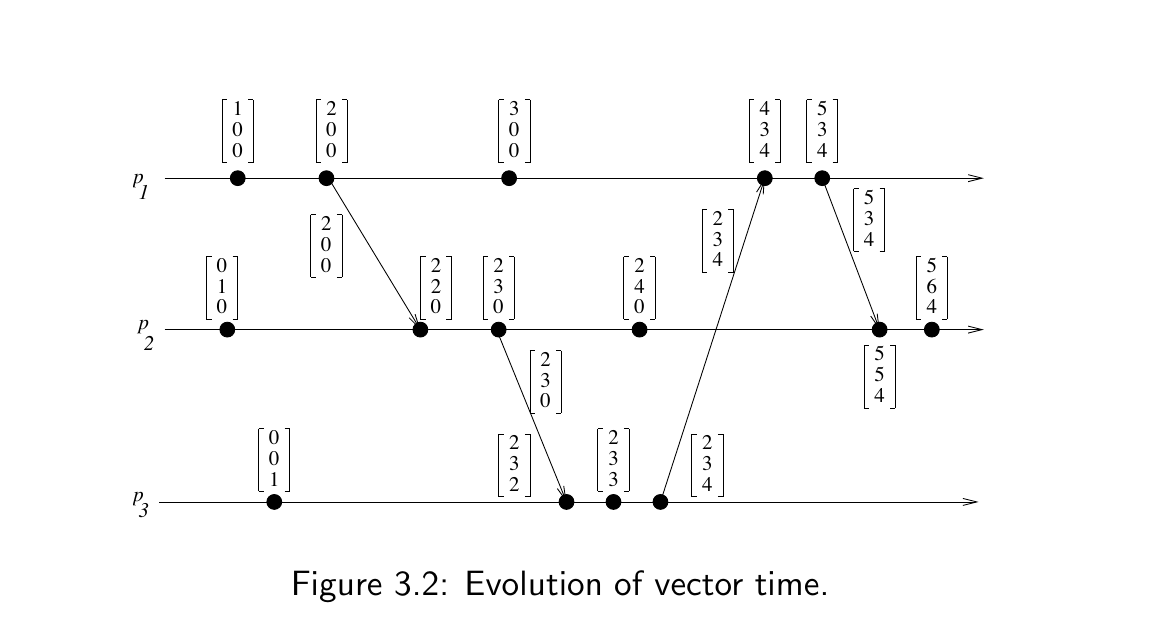
\includegraphics[trim=0 62 0 0,clip,width=\linewidth,height=.51\paperheight,keepaspectratio]{assets/week03-source-2025/vector-time-evolution.png}
\end{center}
\column{.39\textwidth}
\begin{enumerate}
  \item 选取两个有路径的事件；
  \item 验证其向量严格小于；
  \item 选取两个无路径事件；
  \item 找到至少两个交叉分量；
  \item 说明标量时钟为何无法给出同样结论。
\end{enumerate}
\end{columns}
\end{frame}

\sectionframe{高效向量时钟与矩阵时间}{在不牺牲语义的前提下利用更新稀疏性，或进一步表达“知识的知识”。}

\begin{frame}{向量时钟的扩展性问题}
当系统包含数千个进程时：
\begin{itemize}
  \item 每条消息携带 $n$ 个分量，通信开销线性增长；
  \item 即使只有少数进程活跃，也要发送大量未变化的分量；
  \item 每个进程和消息缓冲区都要保存较大的时间戳；
  \item 强一致性在一般情形下仍需要 $n$ 维，因此优化重点是利用实际更新稀疏性。
\end{itemize}
\vfill
\callout{优化问题}{能否只发送“自上次给这个接收者发消息以来发生变化的分量”？}
\end{frame}

\begin{frame}{Singhal--Kshemkalyani 差分技术}
核心观察：对固定的接收者 $p_j$，发送者 $p_i$ 连续两次发送之间通常只有少数向量分量改变。
\begin{itemize}
  \item 不再随消息发送完整 $VT_i$；
  \item 只发送相对上次发给 $p_j$ 后变化的分量；
  \item 用稀疏的 $(\text{索引},\text{最新值})$ 二元组集合编码；
  \item 时空局部性越强，压缩效果越好。
\end{itemize}
\end{frame}

\begin{frame}{差分时间戳的编码形式}
若分量 $i_1,i_2,\ldots,i_r$ 自上次发送给 $p_j$ 后分别变为 $v_1,v_2,\ldots,v_r$，则携带：
\[
\{(i_1,v_1),(i_2,v_2),\ldots,(i_r,v_r)\}.
\]
\begin{itemize}
  \item 最好情况：没有新知识，差分很小；
  \item 常见情况：只发送少量变化分量；
  \item 最坏情况：所有分量都变化，仍需发送完整 $n$ 维信息；
  \item 平均消息开销取决于通信与更新局部性。
\end{itemize}
\end{frame}

\begin{frame}{接收差分时间戳：只更新出现的分量}
若 $p_j$ 收到集合
\[
\{(i_k,v_k)\mid k=1,\ldots,r\},
\]
则执行：
\[
VT_j[i_k]:=\max(VT_j[i_k],v_k),\qquad k=1,\ldots,r.
\]
然后再递增 $VT_j[j]$ 记录接收事件。
\vfill
\callout{收益}{减少消息大小、传输带宽和缓冲区占用；最坏复杂度不变，但平均开销下降。}
\end{frame}

\begin{frame}{朴素差分实现为什么需要 $O(n^2)$ 存储}
发送者要知道“上次给每个接收者发送时，完整向量是什么”：
\begin{itemize}
  \item 对 $n-1$ 个接收者分别保存一个 $n$ 维历史向量；
  \item 每个进程的额外状态因此达到 $O(n^2)$；
  \item 这会抵消消息压缩带来的收益；
  \item Singhal--Kshemkalyani 用两个长度为 $n$ 的向量把状态降为 $O(n)$。
\end{itemize}
\end{frame}

\begin{frame}{$LS_i$ 与 $LU_i$：用“时间”判断分量是否变化}
进程 $p_i$ 维护：
\begin{itemize}
  \item $LS_i[j]$（Last Sent）：上次向 $p_j$ 发送时 $VT_i[i]$ 的值；
  \item $LU_i[k]$（Last Update）：$VT_i[k]$ 最近一次被更新时 $VT_i[i]$ 的值；
  \item 始终有 $LU_i[i]=VT_i[i]$；
  \item 只有收到消息导致 $VT_i[k]$ 增长时，才更新 $LU_i[k]$。
\end{itemize}
\vfill
\callout{压缩状态}{两个 $n$ 维向量足以回答“哪个分量在上次给 $p_j$ 发送之后变化过”。}
\end{frame}

\begin{frame}{选择需要发送的分量}
从 $p_i$ 向 $p_j$ 发送时，只携带满足条件的分量：
\[
\{(x,VT_i[x])\mid LS_i[j]<LU_i[x]\}.
\]
发送后更新：
\[
LS_i[j]:=VT_i[i].
\]
\begin{itemize}
  \item $LU_i[x]$ 晚于 $LS_i[j]$，说明分量 $x$ 在上次发送后改变；
  \item 条件不成立的分量，接收方已经从此前消息获得；
  \item 发送开销与实际变化数相关。
\end{itemize}
\end{frame}

\begin{frame}{为什么差分技术要求 FIFO 信道}
\begin{itemize}
  \item 新消息省略的分量，依赖旧消息已经把基线送达；
  \item 若同一发送者到接收者的消息重排，后发差分可能先到；
  \item 接收者缺少被省略的旧值，无法重建完整知识；
  \item FIFO 保证每个差分都基于接收者已经获得的前一版本。
\end{itemize}
\vfill
\callout{协议教训}{压缩经常引入隐藏前提：省略的数据必须能由可靠、有序的历史恢复。}
\end{frame}

\begin{frame}{差分向量时钟的演化示例}
\begin{center}
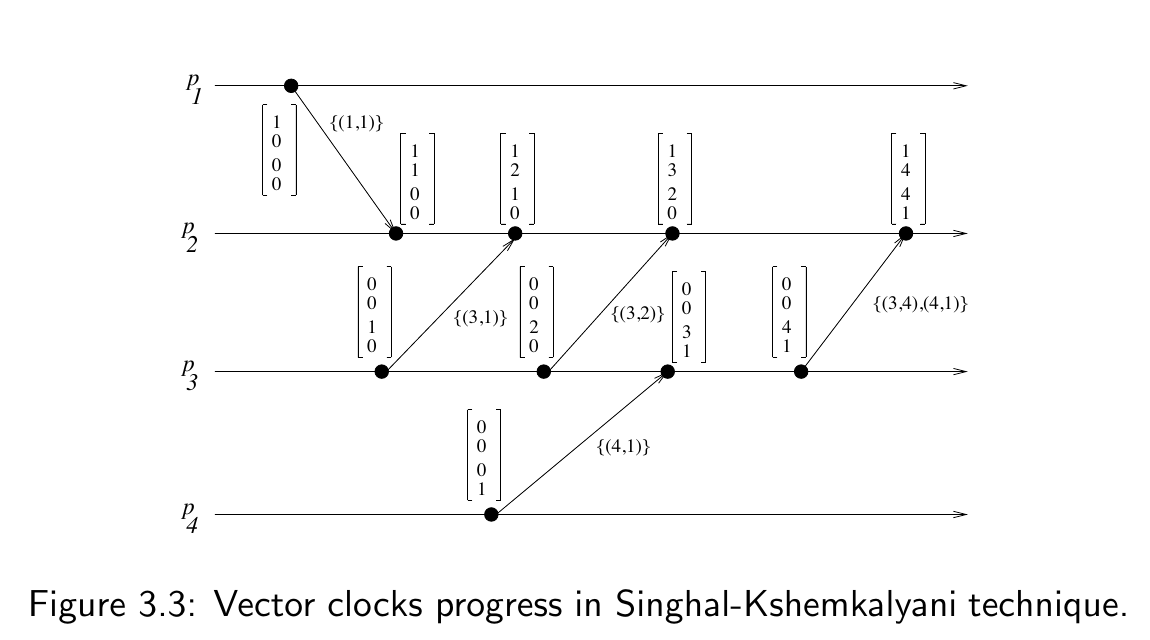
\includegraphics[trim=0 76 0 0,clip,width=.94\linewidth,height=.60\paperheight,keepaspectratio]{assets/week03-source-2025/differential-vector-clock.png}
\end{center}
\smallnote{图示：消息只携带相对同一接收者上次通信后改变的分量。}
\end{frame}

\begin{frame}{示例解读：为什么第二条消息只需携带 $(3,2)$}
$p_3$ 第二次向 $p_2$ 发送时：
\begin{itemize}
  \item 上次消息已让 $p_2$ 知道第三分量为 1；
  \item 此后 $p_3$ 的第三分量从 1 增长到 2；
  \item 其他相关分量没有新的变化；
  \item 因而只发送 $\{(3,2)\}$ 即可恢复与完整向量相同的知识。
\end{itemize}
\vfill
\callout{适用场景}{进程交互具有时间或空间局部性时，差分消息通常远小于完整向量。}
\end{frame}

\begin{frame}{现代工程中的稀疏因果元数据}
差分思想可映射到：
\begin{itemize}
  \item 只记录活跃副本的稀疏版本向量；
  \item dotted version vectors，将单次事件与因果上下文分离；
  \item 增量 checkpoint、增量状态同步与 delta-CRDT；
  \item Trace context 中只传播当前路径需要的依赖信息。
\end{itemize}
\vfill
\smallnote{扩展内容用于联系现代系统；基本语义仍由差分向量时钟给出。}
\end{frame}

\begin{frame}{矩阵时间：从“我知道什么”到“我知道别人知道什么”}
进程 $p_i$ 维护非负整数矩阵：
\[
MT_i[1..n,1..n].
\]
\begin{itemize}
  \item $MT_i[i,i]$：$p_i$ 的本地逻辑时间；
  \item $MT_i[i,j]$：$p_i$ 已知的 $p_j$ 本地时间；
  \item $MT_i[j,k]$：据 $p_i$ 所知，$p_j$ 已知的 $p_k$ 最新时间；
  \item 整个矩阵表达 $p_i$ 对全局逻辑时间与二阶知识的视图。
\end{itemize}
\end{frame}

\begin{frame}{矩阵分量的知识层次}
\begin{center}
\begin{tikzpicture}[node distance=9mm]
\nodebox{ADSBlue}{local}{$MT_i[i,i]$};
\nodebox[right=of local]{ADSOrange}{first}{$MT_i[i,j]$};
\nodebox[right=of first]{ADSGreen}{second}{$MT_i[j,k]$};
\draw[ADSBlue,\arrow] (local)--(first);
\draw[ADSOrange,\arrow] (first)--(second);
\node[below=4mm of local,align=center,text=ADSGray]{我的进展};
\node[below=4mm of first,align=center,text=ADSGray]{我知道 $j$ 的进展};
\node[below=4mm of second,align=center,text=ADSGray]{我知道 $j$ 知道 $k$ 的进展};
\end{tikzpicture}
\end{center}
\vfill
\callout{用途}{二阶知识可用于判断旧信息是否已被所有相关进程越过，从而安全回收。}
\end{frame}

\begin{frame}{矩阵时钟 R1 与 R2}
本地事件前：
\[
MT_i[i,i]:=MT_i[i,i]+d.
\]
收到 $p_j$ 携带的矩阵 $MT$ 后：
\[
\forall k:\ MT_i[i,k]:=\max(MT_i[i,k],MT[j,k]),
\]
并合并整个矩阵：
\[
\forall k,l:\ MT_i[k,l]:=\max(MT_i[k,l],MT[k,l]).
\]
随后执行 R1 并交付消息。
\end{frame}

\begin{frame}{矩阵时间的演化示例}
\begin{center}
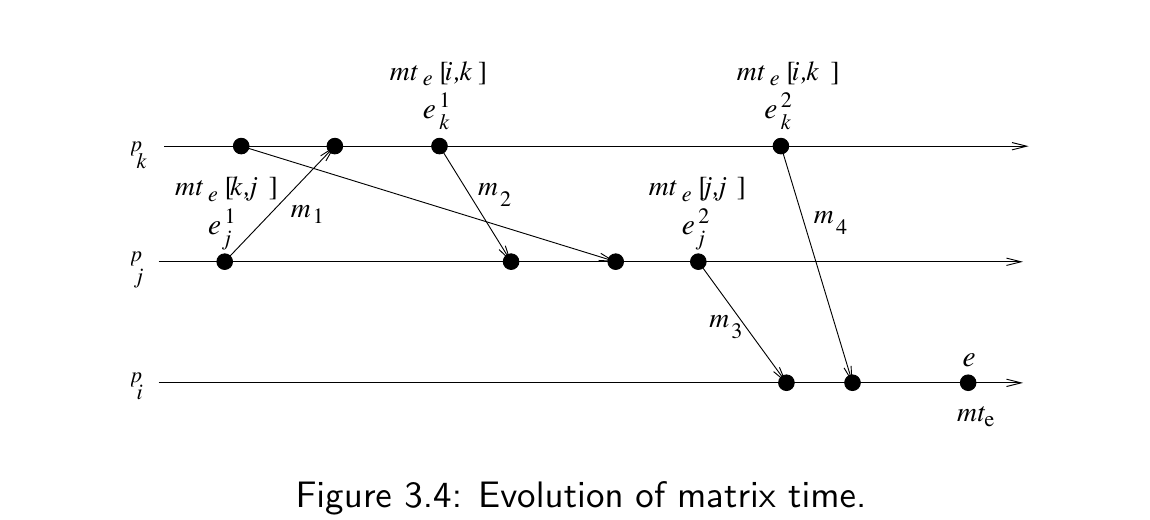
\includegraphics[trim=0 62 0 0,clip,width=.94\linewidth,height=.59\paperheight,keepaspectratio]{assets/week03-source-2025/matrix-time-evolution.png}
\end{center}
\smallnote{图示：矩阵的第 $i$ 行保留向量时钟语义，其他行保存二阶知识。}
\end{frame}

\begin{frame}{如何读 Figure 3.4 中的矩阵分量}
对 $p_i$ 上事件 $e$ 的矩阵时间 $MT_e$：
\begin{itemize}
  \item $MT_e[i,k]$ 是 $p_i$ 已知的 $p_k$ 最新事件位置；
  \item $MT_e[i,j]$ 是 $p_i$ 已知的 $p_j$ 最新事件位置；
  \item $MT_e[j,k]$ 是据 $p_i$ 所知，$p_j$ 对 $p_k$ 的最新知识；
  \item 不同消息路径让这些一阶与二阶知识逐步传播。
\end{itemize}
\end{frame}

\begin{frame}{矩阵时钟的关键性质}
矩阵的第 $i$ 行 $MT_i[i,*]$ 具有向量时钟的全部性质。此外：
\[
\min_k MT_i[k,l]\ge t
\]
意味着 $p_i$ 知道：每个进程 $p_k$ 都知道 $p_l$ 的本地时间至少已到 $t$。
\vfill
\begin{itemize}
  \item $p_i$ 获得了“所有人都已越过 $p_l$ 的时间 $t$”的证据；
  \item 某些早于 $t$ 的信息因此不可能再成为新消息；
  \item 系统可据此回收陈旧日志、消息或状态。
\end{itemize}
\end{frame}

\begin{frame}{矩阵时间与垃圾回收}
\begin{columns}[T,onlytextwidth]
\column{.47\textwidth}
\blocktitle{待回收对象}
\begin{itemize}
  \item 旧版本与 tombstone；
  \item 已处理消息记录；
  \item 仿真中的历史状态；
  \item 检查点之前的日志。
\end{itemize}
\column{.47\textwidth}
\blocktitle{安全条件}
\begin{itemize}
  \item 不仅“我已经处理”；
  \item 还要知道其他进程也不会再引用；
  \item 二阶知识提供全局稳定性的近似证据；
  \item 代价是矩阵级元数据。
\end{itemize}
\end{columns}
\end{frame}

\begin{frame}{标量、向量与矩阵时间：能力与成本}
\begin{tabularx}{\linewidth}{>{\bfseries}p{2.2cm}XXX}
\toprule
 & 标量 & 向量 & 矩阵 \\
\midrule
每进程状态 & $O(1)$ & $O(n)$ & $O(n^2)$ \\
因果一致 & 是 & 是 & 是 \\
强一致 & 否 & 是 & 至少包含向量能力 \\
并发判断 & 否 & 是 & 是 \\
知识层次 & 聚合高度 & 一阶知识 & 二阶知识 \\
典型问题 & 排序 & 依赖/冲突 & 稳定性/回收 \\
\bottomrule
\end{tabularx}
\vfill
\callout{选型原则}{只为实际需要的语义付费；更大的时钟并不自动让系统“更正确”。}
\end{frame}

\sectionframe{Virtual Time 与 Time Warp}{乐观地让各进程向前执行；一旦迟到消息揭示因果冲突，就回滚并撤销错误影响。}

\begin{frame}{Virtual Time：组织和同步分布式仿真的范式}
\begin{itemize}
  \item Virtual Time 用一个应用定义的时间坐标描述计算进度；
  \item 每个逻辑进程可独立推进，不必在每一步全局同步；
  \item Time Warp 是一种乐观实现：先执行，发现冲突后回滚；
  \item 其基本机制是 lookahead--rollback；
  \item 适合离散事件仿真等事件具有明确逻辑时间的系统。
\end{itemize}
\vfill
\callout{与逻辑时钟的区别}{Lamport 时钟从执行中推导标签；Virtual Time 由应用事件自带时间语义，并据此调度执行。}
\end{frame}

\begin{frame}{乐观同步：假设冲突和回滚通常较少}
Time Warp 允许进程暂时不考虑其他进程的同步冲突而继续执行：
\begin{itemize}
  \item 若后续没有更早事件到达，乐观执行直接转化为并行收益；
  \item 若发现冲突，将相关进程回滚到冲突之前；
  \item 从恢复点沿修正后的事件顺序重新向前执行；
  \item 冲突检测与回滚对应用逻辑尽可能透明；
  \item 性能依赖“错误推测的代价”与“并行前进收益”的平衡。
\end{itemize}
\end{frame}

\begin{frame}{Virtual Time 的定义}
Virtual Time 是分布式计算上的一个时间坐标系统，用于：
\begin{itemize}
  \item 度量计算进度；
  \item 定义事件之间的同步条件；
  \item 给事件和消息赋予应用语义上的时间；
  \item 通过多个松散同步的局部虚拟时钟实现。
\end{itemize}
\vfill
局部虚拟时钟通常向前推进，但在乐观执行出错时允许回退。
\end{frame}

\begin{frame}{每条 Virtual Time 消息包含四类信息}
\begin{enumerate}
  \item 发送者名称或虚拟空间坐标；
  \item virtual send time：发送时发送者的虚拟时间；
  \item 接收者名称或虚拟空间坐标；
  \item virtual receive time：消息应被接收和处理的虚拟时间。
\end{enumerate}
\vfill
\callout{调度依据}{接收时间戳而不是物理到达时间决定事件在仿真时间轴上的位置。}
\end{frame}

\begin{frame}{迟到消息：物理到达顺序违反虚拟时间顺序}
若消息到达时：
\[
T_{recv}(m)<LVT_i,
\]
其中 $LVT_i$ 是接收进程当前局部虚拟时间，则消息是 straggler（迟到消息）。
\begin{itemize}
  \item 进程已经执行了逻辑上晚于该消息的事件；
  \item 当前状态可能依赖错误的事件顺序；
  \item 仅把迟到消息插入队列并继续执行是不正确的；
  \item 必须恢复到该消息之前的状态并重新执行。
\end{itemize}
\end{frame}

\begin{frame}{Virtual Time 的两条语义规则}
\begin{enumerate}
  \item 对每条消息：virtual send time $<$ virtual receive time；
  \item 对同一进程的连续事件：前一事件的 virtual time $<$ 后一事件的 virtual time。
\end{enumerate}
它们意味着：
\begin{itemize}
  \item 进程按发送时间递增地产生消息；
  \item 每个进程最终必须按接收时间戳递增处理消息；
  \item 物理到达可以乱序，但最终提交的逻辑执行不能乱序。
\end{itemize}
\end{frame}

\begin{frame}{因果约束：原因必须在真实执行中先完成}
若事件 $A$ 导致事件 $B$：
\[
A\rightarrow B,
\]
则真实执行调度必须保证 $A$ 完成后才能使 $B$ 成为最终有效结果。
\vfill
\begin{itemize}
  \item 乐观系统可以暂时执行 $B$；
  \item 但若后来发现遗漏了 $A$ 或其前驱，就必须撤销 $B$；
  \item 回滚把“临时违反”修正为“最终符合”因果顺序；
  \item 因此正确性基于可撤销执行，而非从不犯错。
\end{itemize}
\end{frame}

\begin{frame}{Virtual Time 的数值先后与因果先后不是一回事}
需要修正一个容易误读的表述：
\begin{itemize}
  \item 若 $A\rightarrow B$，必须保证 $A$ 的有效执行先于 $B$；
  \item 若 $VT(A)<VT(B)$ 但 $A$ 与 $B$ 无因果关系，可并行或按任意物理顺序推测执行；
  \item 若二者虚拟时间相同且属于不同逻辑进程，通常也不存在由时间值本身产生的顺序约束；
  \item 系统最终只需让每个逻辑进程的已提交事件符合其时间戳顺序和因果约束。
\end{itemize}
\vfill
\callout{语义提醒}{时间戳数值顺序不能替代因果关系；本页按 Time Warp 的标准语义表述。}
\end{frame}

\begin{frame}{Virtual Time 系统的可选特征}
\begin{itemize}
  \item 时间域可以离散，也可以连续；
  \item 时间关系可以全序，也可以只定义偏序；
  \item 虚拟时间可以映射现实时间，也可以完全独立；
  \item 时间值可以显式暴露给程序员，也可以由运行时隐式维护；
  \item 时间戳可以由应用计算，也可以由固定系统规则分配。
\end{itemize}
\end{frame}

\begin{frame}{Time Warp 与 Lamport 时钟的对照}
\begin{tabularx}{\linewidth}{>{\bfseries}p{2.6cm}XX}
\toprule
 & Lamport 逻辑时钟 & Virtual Time / Time Warp \\
\midrule
时间来源 & 从已有执行和消息关系推导 & 应用事件预先带有虚拟时间 \\
推进方式 & 保守更新，始终保持因果单调 & 乐观推进，发现冲突后修正 \\
回退 & 不需要 & 局部时钟和状态可回退 \\
核心目标 & 标记因果顺序 & 并行执行时间戳事件 \\
错误处理 & 更新时避免违反 & 通过回滚撤销违反 \\
\bottomrule
\end{tabularx}
\end{frame}

\begin{frame}{Time Warp 的核心难题：无法仅凭局部信息等待“下一条”}
\begin{itemize}
  \item 进程速度和消息延迟高度可变；
  \item 信道可靠但允许 Non-FIFO 交付；
  \item 当前队首的时间戳最小，不代表未来不会到达更小时间戳；
  \item 若一味阻塞等待，进程无法知道何时已经安全；
  \item Time Warp 选择立即处理当前最小事件，并为可能的回滚保留证据。
\end{itemize}
\end{frame}

\begin{frame}{Time Warp 的两部分控制机制}
\begin{columns}[T,onlytextwidth]
\column{.47\textwidth}
\blocktitle{局部控制}
\begin{itemize}
  \item 按时间戳处理输入事件；
  \item 检测迟到消息；
  \item 保存状态并执行回滚；
  \item 发送反消息撤销输出。
\end{itemize}
\column{.47\textwidth}
\blocktitle{全局控制}
\begin{itemize}
  \item 估计全局进展；
  \item 判断终止；
  \item 安全提交 I/O；
  \item 流量控制与历史回收。
\end{itemize}
\end{columns}
\end{frame}

\begin{frame}{局部虚拟时钟：只在事件之间跳转}
\begin{itemize}
  \item 系统中没有单一全局虚拟时钟变量；
  \item 每个逻辑进程维护自己的 $LVT_i$；
  \item 处理一个事件期间，$LVT_i$ 保持为该事件的时间戳；
  \item 取出下一条消息时，$LVT_i$ 跳到消息的 virtual receive time；
  \item 不同进程的 $LVT$ 可以相差很大，对其他进程透明。
\end{itemize}
\end{frame}

\begin{frame}{输入队列：按虚拟接收时间排序}
到达进程的消息存入输入队列：
\begin{itemize}
  \item 队列按 virtual receive time 递增排序；
  \item 物理到达顺序不必与队列顺序一致；
  \item 已处理消息暂时不能删除，因为未来回滚可能需要重新处理；
  \item 若新到消息时间戳小于 $LVT_i$，触发回滚；
  \item 正确性要求最终有效执行按时间戳顺序。
\end{itemize}
\end{frame}

\begin{frame}{一个 Time Warp 进程需要保存什么}
\begin{tabularx}{\linewidth}{>{\bfseries}p{2.6cm}X}
\toprule
运行时对象 & 作用 \\
\midrule
进程名 & 唯一虚拟空间坐标 \\
局部虚拟时钟 & 当前处理事件的时间坐标 \\
当前状态 & 栈、程序计数器和应用变量 \\
状态队列 & 保存近期状态，用于回滚恢复 \\
输入队列 & 保存近期到达和已处理消息 \\
输出队列 & 保存已发送消息的负副本，即反消息 \\
\bottomrule
\end{tabularx}
\vfill
\callout{空间换时间}{乐观并行必须保存足够历史，才能撤销错误推测。}
\end{frame}

\begin{frame}{反消息：撤销一个已经发送的消息}
每条正消息都有内容相同、符号相反的 antimessage：
\begin{itemize}
  \item 发送正消息时，正副本进入接收方输入队列；
  \item 负副本保留在发送方输出队列；
  \item 正消息与对应反消息在同一队列相遇时立即湮灭；
  \item 若发送方回滚到发送之前，就把反消息发往接收方；
  \item 反消息负责撤销错误执行向其他进程传播的影响。
\end{itemize}
\end{frame}

\begin{frame}{回滚机制：恢复状态、撤销输出、重新前进}
收到迟到消息 $m$ 后：
\begin{enumerate}
  \item 在状态队列中找到时间戳小于 $T_{recv}(m)$ 的最近状态；
  \item 恢复该状态，并将 $LVT$ 调整到相应位置；
  \item 丢弃该时间之后保存的状态；
  \item 对回滚区间内发出的每条消息发送其反消息；
  \item 把迟到消息放入正确位置，从恢复点重新执行。
\end{enumerate}
\vfill
\callout{撤销规则}{“取消发送一条消息”的实现，就是发送它的反消息。}
\end{frame}

\begin{frame}{完整例子：三条虚拟时间线}
\begin{center}
\resizebox{.98\linewidth}{!}{%
\begin{tikzpicture}[>=Latex,x=0.15cm,y=1cm]
  \draw[ADSGray,->] (0,0)--(75,0) node[right,font=\scriptsize]{虚拟时间};
  \draw[ADSGray,->] (0,-1.4)--(75,-1.4);
  \draw[ADSGray,->] (0,-2.8)--(75,-2.8);
  \node[anchor=east,font=\scriptsize] at (-1,0){$p_1$};
  \node[anchor=east,font=\scriptsize] at (-1,-1.4){$p_2$};
  \node[anchor=east,font=\scriptsize] at (-1,-2.8){$p_3$};
  \foreach \t in {10,20,25,30,35,40,50,60}{\draw[ADSGray] (\t,0.08)--(\t,-0.08) node[below,font=\tiny]{\t};}
  \draw[ADSBlue,very thick] (10,0) circle (2pt) node[above,font=\scriptsize]{send $m$};
  \draw[ADSOrange,very thick] (20,-1.4) circle (2pt) node[above,font=\scriptsize]{state $S_{20}$};
  \draw[ADSOrange,very thick] (30,-1.4) circle (2pt) node[above,font=\scriptsize]{send $x$};
  \draw[ADSOrange,very thick] (40,-1.4) circle (2pt) node[above,font=\scriptsize]{LVT=40};
  \draw[ADSGreen,very thick] (35,-2.8) circle (2pt) node[below,font=\scriptsize]{处理 $x$};
  \draw[ADSBlue,thick,->] (10,-.15) .. controls (16,-.65) and (20,-.8) .. (25,-1.25) node[midway,above,font=\scriptsize]{应在 25 接收};
  \draw[ADSOrange,thick,->] (30,-1.55) .. controls (33,-2.0) and (34,-2.3) .. (35,-2.65) node[midway,right,font=\scriptsize]{物理到达};
  \end{tikzpicture}}
\end{center}
\begin{itemize}
  \item $p_2$ 先乐观执行到 40；消息 $m$ 的虚拟接收时间是 25，却在物理上晚到；
  \item 因此 $m$ 是 straggler，$p_2$ 之前在 30 产生的 $x$ 也可能需要撤销。
\end{itemize}
\end{frame}

\begin{frame}{完整例子 Step 1：先执行“看起来安全”的事件}
\begin{tabularx}{\linewidth}{>{\bfseries}p{2.7cm}XX}
\toprule
虚拟时间 & $p_2$ 的状态 & 已发送/已处理 \\
20 & 保存检查点 $S_{20}$ & 无 \\
30 & 更新状态并发送 $x$ 给 $p_3$，$T_{recv}(x)=35$ & $x$ 进入输出队列 \\
40 & 继续本地事件，$LVT_2=40$ & 认为到目前为止没有冲突 \\
\bottomrule
\end{tabularx}
\vfill
\callout{为什么允许这样做}{若 $m$ 最终不存在，等待它只会浪费并行度；Time Warp 选择先执行，同时保存足够的回滚证据。}
\end{frame}

\begin{frame}{完整例子 Step 2：迟到消息触发回滚}
现在 $m$ 到达 $p_2$，且 $T_{recv}(m)=25<LVT_2=40$：
\begin{enumerate}
  \item 在状态队列中找到最近的 $S_{20}$；
  \item 恢复 $S_{20}$，丢弃虚拟时间 20 之后的临时状态；
  \item 对 30 时发送的 $x$ 生成反消息 $\overline{x}$；
  \item 把 $m$ 放回时间 25 的输入位置，重新执行后续事件。
\end{enumerate}
\vfill
\smallnote{回滚不是“把时钟减回去就结束”，还必须撤销已经传播给其他进程的输出。}
\end{frame}

\begin{frame}{完整例子 Step 3：反消息如何影响 $p_3$}
\begin{columns}[T,onlytextwidth]
\column{.47\textwidth}
\blocktitle{$x$ 尚未处理}
\begin{itemize}
  \item $x$ 和 $\overline{x}$ 在输入队列相遇；
  \item 两者直接湮灭；
  \item $p_3$ 不需要回滚。
\end{itemize}
\column{.47\textwidth}
\blocktitle{$x$ 已在 35 处理}
\begin{itemize}
  \item $p_3$ 回滚到处理 $x$ 之前；
  \item 撤销由 $x$ 派生的输出；
  \item 等待 $p_2$ 重新发送修正后的结果。
\end{itemize}
\end{columns}
\vfill
\callout{本例}{由于 $p_3$ 已在 35 处理 $x$，$\overline{x}$ 会沿因果链触发一次局部回滚。}
\end{frame}

\begin{frame}{完整例子 Step 4：从 20 重新前进}
\begin{enumerate}
  \item $p_2$ 在 25 处理迟到消息 $m$，得到修正状态；
  \item $p_2$ 重新执行 30 时事件，产生 $x'$；
  \item $x'$ 可能与旧 $x$ 内容不同，但拥有新的消息实例 ID；
  \item $p_3$ 在 35 处理 $x'$，其状态与 $p_2$ 的因果历史一致；
  \item 当后续没有更早消息时，两个进程继续向前推进。
\end{enumerate}
\vfill
\callout{关键点}{Time Warp 最终保留的是“修正后的一次有效执行”，而不是把错误执行永久写入外部世界。}
\end{frame}

\begin{frame}{完整例子 Step 5：GVT 与历史回收}
假设某一时刻：
\begin{itemize}
  \item $LVT_1=50$，$LVT_2=45$，$LVT_3=60$；
  \item 网络中最早的未处理消息时间戳为 38；
  \item 则可以取 $GVT=\min(50,45,60,38)=38$。
\end{itemize}
\begin{enumerate}
  \item 时间小于 38 的状态不再可能被迟到消息影响；
  \item 可以提交相应的外部 I/O；
  \item 可以回收早于 38 的状态、正消息和反消息；
  \item 仍需保留时间等于或大于 38 的历史。
\end{enumerate}
\vfill
\callout{工程含义}{GVT 同时是“安全提交线”和“垃圾回收线”；估计 GVT 本身又需要分布式协调。}
\end{frame}

\begin{frame}{完整例子的最终时间线}
\begin{center}
\resizebox{.96\linewidth}{!}{%
\begin{tikzpicture}[>=Latex,x=0.16cm,y=1cm]
  \draw[ADSGray,->] (0,0)--(70,0) node[right,font=\scriptsize]{修正后的虚拟执行};
  \foreach \t in {20,25,30,35,38,45,50,60}{\draw[ADSGray] (\t,0.08)--(\t,-0.08) node[below,font=\tiny]{\t};}
  \draw[ADSOrange,very thick] (20,0) circle (2pt) node[above,font=\scriptsize]{$S_{20}$};
  \draw[ADSBlue,very thick] (25,0) circle (2pt) node[above,font=\scriptsize]{$m$};
  \draw[ADSGreen,very thick] (30,0) circle (2pt) node[above,font=\scriptsize]{$x'$};
  \draw[ADSGray,dashed,very thick] (38,-.4)--(38,.4) node[above,font=\scriptsize]{GVT};
  \draw[ADSGray,very thick] (45,0) circle (2pt) node[above,font=\scriptsize]{继续};
  \draw[ADSGray,very thick] (60,0) circle (2pt) node[above,font=\scriptsize]{继续};
  \draw[ADSOrange,decorate,decoration={brace,mirror,amplitude=4pt}] (0,-.55)--(38,-.55) node[midway,below=5pt,font=\scriptsize]{可提交与回收};
  \end{tikzpicture}}
\end{center}
\begin{itemize}
  \item 错误的 $x$ 和其反消息属于临时历史；有效结果是 $x'$；
  \item 只有越过 GVT 的结果才能安全对外部系统承诺。
\end{itemize}
\end{frame}

\begin{frame}{接收端情形一：正消息尚未处理}
若正消息已经到达但仍在输入队列中：
\begin{itemize}
  \item 反消息到达后与正消息直接湮灭；
  \item 接收进程没有基于该消息执行任何事件；
  \item 因而不需要状态回滚；
  \item 队列中也不再保留该消息的记录。
\end{itemize}
\end{frame}

\begin{frame}{接收端情形二：正消息已经被处理}
若接收方已经部分或全部处理正消息：
\begin{itemize}
  \item 反消息触发接收方回滚到处理该正消息之前；
  \item 正消息与反消息湮灭；
  \item 接收方重新执行时，相当于该消息从未存在；
  \item 接收方此前发送的派生消息也要通过更多反消息撤销；
  \item 因此一次回滚可能沿因果链传播。
\end{itemize}
\end{frame}

\begin{frame}{接收端情形三：反消息先于正消息到达}
\begin{itemize}
  \item 反消息先进入输入队列等待对应正消息；
  \item 正消息到达时二者湮灭；
  \item 若运行时轮到反消息，可把它视为 no-op；
  \item 即使暂时执行了其他动作，正消息到达后仍可通过回滚修正；
  \item 优化实现会跳过孤立反消息，减少无意义回滚。
\end{itemize}
\end{frame}

\begin{frame}{反消息协议的性质}
\begin{itemize}
  \item 对正负消息各种到达顺序都能工作；
  \item 不通过阻塞等待同步，因此不会形成等待型死锁；
  \item 通过精确的消息撤销避免检查点系统中的无界 domino rollback；
  \item 最坏情况下多个进程可能回滚到较早虚拟时间后重新执行；
  \item 稳定性与性能依赖状态保存、取消机制和流量控制。
\end{itemize}
\end{frame}

\begin{frame}{Global Virtual Time：什么历史已经不可能被回滚}
扩展概念 GVT 可理解为系统中所有未完成工作的最小虚拟时间下界：
\begin{itemize}
  \item 时间早于 GVT 的事件不再可能被迟到消息撤销；
  \item 可安全提交对应外部 I/O；
  \item 可回收早于 GVT 的状态、消息和反消息；
  \item 可用于度量全局进展和辅助终止检测；
  \item 其计算本身又是一次分布式全局状态问题。
\end{itemize}
\end{frame}

\begin{frame}{课堂互动：手工执行一次 Time Warp 回滚}
\begin{columns}[T,onlytextwidth]
\column{.47\textwidth}
\blocktitle{场景}
\begin{itemize}
  \item $p_2$ 已执行时间 20、30、40 的事件；
  \item 时间 40 的事件向 $p_3$ 发送消息 $x$；
  \item 此时收到 virtual receive time 为 25 的消息 $m$。
\end{itemize}
\column{.47\textwidth}
\blocktitle{任务}
\begin{enumerate}
  \item 选择恢复状态；
  \item 标出被撤销事件；
  \item 生成 $x$ 的反消息；
  \item 分析 $p_3$ 的三种可能状态；
  \item 判断哪些历史尚不能回收。
\end{enumerate}
\end{columns}
\end{frame}

\sectionframe{物理时钟同步与 NTP}{逻辑时间保持因果；需要现实时间、跨机区间和审计时间线时，还必须估计物理时钟误差。}

\begin{frame}{物理时钟同步的动机}
集中式系统通常由内核提供一个时钟；分布式系统中每台机器都有独立振荡器：
\begin{itemize}
  \item 没有全局时钟和公共内存；
  \item 各时钟的初始 offset 不同；
  \item 频率略有差异，误差会随时间积累；
  \item 即使启动时同步，运行后也会逐渐分离；
  \item 每天漂移数秒就足以破坏许多时间敏感应用。
\end{itemize}
\end{frame}

\begin{frame}{分布式应用为什么需要物理时间}
常见问题包括：
\begin{enumerate}
  \item 某台机器上的事件发生于现实世界的什么时间？
  \item 两台机器上的事件相隔多长时间？
  \item 两个跨机事件的现实时间先后是什么？
\end{enumerate}
\vfill
时钟同步影响安全系统、故障诊断与恢复、定时任务、数据库、监控告警、证书有效期和审计日志。
\vfill
\callout{边界}{物理时间有误差区间；在要求严格因果的场合，不能只比较两个墙上时间戳。}
\end{frame}

\begin{frame}{物理时钟同步：共同接近 UTC}
\begin{itemize}
  \item 时钟同步让分散处理器具有近似共同的时间尺度；
  \item 由于频率误差，需要周期性重新校准；
  \item 常见参考标准为 UTC；
  \item 只要求节点彼此接近称为内部同步；
  \item 还要求接近外部真实时间标准称为外部同步；
  \item 与 UTC 对齐的时钟属于物理时钟系统。
\end{itemize}
\end{frame}

\begin{frame}{基本术语：时间、频率与 offset}
令机器 $p$ 的时钟读数为 $C_p(t)$，其中 $t$ 是理想参考时间：
\begin{itemize}
  \item 完美时钟：$C_p(t)=t$；
  \item 频率：$\dot C_p(t)$，表示时钟推进速度；
  \item 对真实时间的 offset：$C_a(t)-t$；
  \item 两时钟的相对 offset：$C_a(t)-C_b(t)$；
  \item offset 是“当前差多少”，频率决定“差距如何增长”。
\end{itemize}
\end{frame}

\begin{frame}{基本术语：skew 与 drift}
\begin{itemize}
  \item 相对 skew：$\dot C_a(t)-\dot C_b(t)$，即频率差；
  \item 相对 drift：$\ddot C_a(t)-\ddot C_b(t)$，即频率差变化率；
  \item offset 可以通过一次校时暂时修正；
  \item skew 会让修正后的时钟再次逐渐分离；
  \item drift 说明 skew 本身也会随温度、老化和负载变化。
\end{itemize}
\vfill
\callout{诊断视角}{看到固定误差先怀疑 offset；误差线性增长先怀疑 skew；增长率变化再考虑 drift。}
\end{frame}

\begin{frame}{制造规格中的最大频率误差}
若时钟最大 skew rate 为 $\rho$，合格时钟满足：
\[
1-\rho\le \frac{dC}{dt}\le 1+\rho.
\]
\begin{itemize}
  \item $dC/dt>1$：快钟；
  \item $dC/dt=1$：理想时钟；
  \item $dC/dt<1$：慢钟；
  \item 两个最坏方向的时钟可按约 $2\rho$ 的速率分离。
\end{itemize}
\end{frame}

\begin{frame}{快钟、慢钟与理想时钟}
\begin{center}
\begin{tikzpicture}[font=\small,>=Latex,scale=.90,transform shape]
  \draw[->,ADSGray] (0,0)--(8,0) node[right]{UTC 参考时间 $t$};
  \draw[->,ADSGray] (0,0)--(0,4.8) node[above,align=center]{本地时钟\\读数 $C(t)$};
  \draw[ADSOrange,line width=1.2pt] (0,0)--(2.4,4.4);
  \draw[ADSBlue,line width=1.2pt] (0,0)--(4.4,4.4);
  \draw[ADSGreen,line width=1.2pt] (0,0)--(7.0,4.0);
  \node[text=ADSOrange,align=center] at (2.0,4.55) {快钟\\$\mathrm dC/\mathrm dt>1$};
  \node[text=ADSBlue,align=center] at (4.4,3.35) {理想时钟\\$\mathrm dC/\mathrm dt=1$};
  \node[text=ADSGreen,align=center] at (7.05,3.75) {慢钟\\$\mathrm dC/\mathrm dt<1$};
  \draw[dashed,ADSGray] (4.4,0)--(4.4,4.4);
  \node[text=ADSGray,font=\scriptsize,align=center] at (5.9,1.1) {斜率偏差会随时间\\累积为时钟误差};
\end{tikzpicture}
\end{center}
\smallnote{图示：纵轴为本地时钟读数，横轴为 UTC 参考时间。}
\end{frame}

\begin{frame}{同步周期与误差预算}
若两时钟最大相对分离速率约为 $2\rho$，希望二者差值不超过 $D$，则同步周期需近似满足：
\[
\Delta t\le \frac{D}{2\rho}.
\]
\begin{itemize}
  \item 更高精度需要更频繁同步；
  \item 网络测量误差会进一步消耗误差预算；
  \item 校时算法还要决定直接 step 还是逐渐 slew；
  \item 真实保证应给出区间或置信度，而不是假装时间戳绝对精确。
\end{itemize}
\end{frame}

\begin{frame}{NTP：基于 offset--delay estimation 的互联网时间协议}
NTP 采用分层时间服务结构：
\begin{itemize}
  \item 顶层时间源直接或间接与 UTC 标准相连；
  \item 次级服务器从上层同步，并为下层提供服务；
  \item 客户端通过网络交换带时间戳的消息估计 offset 与 delay；
  \item 多个服务器和多轮样本用于容错与滤除异常；
  \item 关键难点是未知且变化的双向网络延迟。
\end{itemize}
\end{frame}

\begin{frame}{四时间戳测量：源页采用的记号}
\begin{center}
\begin{tikzpicture}[font=\small,>=Latex,scale=.92,transform shape]
  \draw[->,ADSGray,line width=1pt] (0,0)--(9,0) node[right]{进程 A 的本地时间};
  \draw[->,ADSGray,line width=1pt] (0,3.8)--(9,3.8) node[right]{进程 B 的本地时间};
  \draw[\arrow,ADSBlue] (2.2,0)--(3.5,3.8);
  \draw[\arrow,ADSOrange] (5.2,3.8)--(6.7,0);
  \foreach \x/\y/\lab in {2.2/0/T_3,3.5/3.8/T_1,5.2/3.8/T_2,6.7/0/T_4}
    {\fill[ADSBlue] (\x,\y) circle (2pt) node[above=2mm] {$\lab$};}
  \node[text=ADSBlue] at (2.4,2.2) {请求};
  \node[text=ADSOrange] at (6.2,2.2) {回复};
  \node[text=ADSGray,font=\scriptsize] at (4.35,.75) {A 记录发送与接收时刻};
  \node[text=ADSGray,font=\scriptsize] at (4.35,3.15) {B 在回复中携带接收与发送时刻};
\end{tikzpicture}
\end{center}
\smallnote{图示：A 在 $T_3$ 发送，B 在 $T_1$ 接收并于 $T_2$ 回复，A 在 $T_4$ 收到。}
\end{frame}

\begin{frame}{从四个时间戳估计 offset 与往返 delay}
令：
\[
a=T_1-T_3,qquad b=T_2-T_4.
\]
若 A$\rightarrow$B 与 B$\rightarrow$A 的单向延迟近似相等，则 B 相对 A 的 offset 与往返 delay 为：
\[
\theta\approx\frac{a+b}{2},
\qquad
\delta\approx a-b.
\]
等价地：
\[
\delta=(T_4-T_3)-(T_2-T_1).
\]
\end{frame}

\begin{frame}{公式推导：把网络延迟与时钟偏移分开}
设 A 到 B、B 到 A 的单向延迟都近似为 $d$，B 的时钟比 A 快 $\theta$：
\[
T_1=T_3+d+\theta,
\]
\[
T_4=T_2+d-\theta.
\]
因此：
\[
T_1-T_3=d+\theta,qquad T_2-T_4=\theta-d.
\]
两式相加消去 $d$ 得 $\theta$，相减消去 $\theta$ 得往返延迟 $2d$。
\end{frame}

\begin{frame}{单向延迟不对称会怎样}
若 A$\rightarrow$B 延迟为 $d_1$，B$\rightarrow$A 延迟为 $d_2$，则估计误差为：
\[
\hat\theta-\theta=\frac{d_1-d_2}{2}.
\]
\begin{itemize}
  \item 四时间戳可以准确测得往返路径总成本；
  \item 但不能仅凭一次交换分离两个单向延迟；
  \item 路径不对称越大，offset 估计偏差越大；
  \item 因此 NTP 使用多次采样，并偏好 delay 更小的样本。
\end{itemize}
\end{frame}

\begin{frame}{双向消息流中的连续时间戳}
\begin{center}
\begin{tikzpicture}[font=\small,>=Latex,scale=.88,transform shape]
  \draw[->,ADSGray,line width=1pt] (0,3.8)--(10,3.8) node[right]{服务器 A};
  \draw[->,ADSGray,line width=1pt] (0,0)--(10,0) node[right]{服务器 B};
  \draw[\arrow,ADSBlue] (1.0,3.8)--(2.4,0);
  \draw[\arrow,ADSOrange] (3.0,0)--(4.4,3.8);
  \draw[\arrow,ADSBlue] (6.0,3.8)--(7.4,0);
  \draw[\arrow,ADSOrange] (8.0,0)--(9.4,3.8);
  \foreach \x/\y/\lab in {2.4/0/T_{i-3},4.4/3.8/T_{i-2},6.0/3.8/T_{i-1},7.4/0/T_i}
    {\fill[ADSBlue] (\x,\y) circle (2pt) node[above=2mm] {$\lab$};}
  \node[text=ADSGray,font=\scriptsize,align=center] at (5,1.85) {双方持续交换时间消息；每次到达都补齐第四个本地时间戳，\\下一次发送再携带最近三项历史。};
\end{tikzpicture}
\end{center}
\smallnote{图示：每条消息携带最近三个时间戳，第四个时间戳在本地到达时获得。}
\end{frame}

\begin{frame}{对称模式：双方持续交换时间消息}
一对 NTP 服务器可在 symmetric mode 下持续交换消息：
\begin{itemize}
  \item 每轮得到一对 $(O_i,D_i)$；
  \item $O_i$ 是该轮估计的 offset；
  \item $D_i$ 是该轮估计的往返传输 delay；
  \item 运行时保留最近若干轮样本；
  \item 一种实用策略是“保留最近 8 对，选择最小 delay 对应的 offset”。
\end{itemize}
\vfill
\callout{直觉}{排队越少，往返 delay 越接近传播下界，路径不确定性通常越小。}
\end{frame}

\begin{frame}{教材记号下的 offset 推导}
设 A、B 的时钟满足：
\[
A(t)=B(t)+O.
\]
对一轮双向交换：
\[
T_{i-2}=T_{i-3}+t+O,
\]
\[
T_i=T_{i-1}-O+t'.
\]
若假设 $t=t'$，则：
\[
O_i=\frac{T_{i-2}-T_{i-3}+T_{i-1}-T_i}{2}.
\]
\end{frame}

\begin{frame}{教材记号下的往返 delay 推导}
同一轮交换的 round-trip delay 估计为：
\[
D_i=(T_i-T_{i-3})-(T_{i-1}-T_{i-2}).
\]
\begin{itemize}
  \item 第一项是 A 观察到的完整往返区间；
  \item 第二项是 B 在两条消息之间的本地处理区间；
  \item 相减后得到两段网络传输时间之和；
  \item 从最近样本中选最小 $D_i$ 对应的 $O_i$ 作为 offset 估计。
\end{itemize}
\end{frame}

\begin{frame}{NTP 能提供什么，不能提供什么}
\begin{columns}[T,onlytextwidth]
\column{.47\textwidth}
\blocktitle{可以提供}
\begin{itemize}
  \item 接近 UTC 的墙上时间；
  \item 毫秒级或更好精度的常见网络同步；
  \item offset、delay、jitter 等质量指标；
  \item 多时间源选择与容错。
\end{itemize}
\column{.47\textwidth}
\blocktitle{不能保证}
\begin{itemize}
  \item 任意网络下的精确单向延迟；
  \item 两个近邻时间戳必然反映因果；
  \item 无误差的全局绝对时间；
  \item 遭遇恶意时间源时自动安全。
\end{itemize}
\end{columns}
\end{frame}

\begin{frame}{从 NTP 到 PTP 与混合逻辑时钟}
\begin{itemize}
  \item PTP 通过硬件时间戳与受控网络追求更高物理同步精度；
  \item TrueTime 类接口显式返回时间不确定区间；
  \item Hybrid Logical Clock 将近似物理时间与逻辑计数结合；
  \item HLC 保持因果单调，同时让时间戳接近墙上时间；
  \item 选型取决于审计、事务、监控、控制和复制协议的实际误差预算。
\end{itemize}
\vfill
\smallnote{扩展内容用于连接现代数据库、云平台和 AI 基础设施。}
\end{frame}

\begin{frame}{AI 基础设施中的时间问题}
\begin{itemize}
  \item 分布式训练 trace 需要跨 GPU/节点对齐时间线；
  \item collective timeout 同时依赖墙上时间与因果证据；
  \item checkpoint 版本应携带逻辑 epoch，不能只依赖文件修改时间；
  \item 推理服务的尾延迟分析需要估计时钟误差；
  \item 调度器事件、指标与日志应通过 trace/span 关系补充物理时间排序。
\end{itemize}
\vfill
\callout{实践建议}{时间戳用于定位区间，消息与 Trace 因果用于证明执行关系。}
\end{frame}

\begin{frame}{本讲知识图谱}
\begin{center}
\begin{tikzpicture}[node distance=7mm]
\nodebox{ADSBlue}{hb}{happened-before};
\nodebox[right=of hb]{ADSOrange}{scalar}{标量时钟};
\nodebox[right=of scalar]{ADSGreen}{vector}{向量时钟};
\nodebox[right=of vector]{ADSGray}{matrix}{矩阵时钟};
\draw[ADSBlue,\arrow] (hb)--(scalar);
\draw[ADSOrange,\arrow] (scalar)--(vector);
\draw[ADSGreen,\arrow] (vector)--(matrix);
\nodebox[below=12mm of scalar]{ADSOrange}{warp}{Time Warp};
\nodebox[right=of warp]{ADSGreen}{ntp}{NTP};
\draw[ADSOrange,\arrow] (scalar)--(warp);
\draw[ADSGreen,\arrow] (warp)--(ntp);
\end{tikzpicture}
\end{center}
\vfill
\smallnote{上行逐步增强因果知识；下行分别处理乐观虚拟时间与现实物理时间。}
\end{frame}

\begin{frame}{本讲总结}
\begin{itemize}
  \item 逻辑时钟的基本条件是 $e\rightarrow f\Rightarrow C(e)<C(f)$；
  \item Lamport 标量时间可构造全序，但不能判断并发；
  \item 向量时间与因果偏序同构，代价为 $O(n)$；
  \item 差分技术利用局部性压缩消息，但依赖 FIFO；
  \item 矩阵时间表达二阶知识，可支持稳定性判断和历史回收；
  \item Time Warp 用回滚与反消息修正乐观执行；
  \item NTP 通过四时间戳估计 offset 与 delay，但受路径不对称限制。
\end{itemize}
\end{frame}

\begin{frame}{课堂互动：选择正确的时间模型}
为下列系统分别选择标量、向量、矩阵、Virtual Time、NTP/PTP 或组合，并说明理由：
\begin{enumerate}
  \item 分布式互斥请求排序；
  \item 多主键值库的版本冲突检测；
  \item 离散事件网络仿真；
  \item 跨机 GPU kernel trace 对齐；
  \item 判断旧 tombstone 是否可安全回收；
  \item 云数据库中既接近墙上时间又保持因果单调的事务时间戳。
\end{enumerate}
\vfill
\callout{回答格式}{需要表达的关系、时间结构、更新规则、开销、不能保证的性质。}
\end{frame}

\begin{frame}{时间模型的三个边界提醒}
\small
\begin{enumerate}
  \item \key{向量时钟：}只比较一个分量不能判断因果；必须做完整的逐分量比较。\(V\leq W\) 且至少一个分量严格小，才表示因果先行；互不支配才表示并发。
  \item \key{矩阵时钟：}课堂图示采用“知识矩阵”的教学化更新；实际协议必须明确是合并完整矩阵，还是只更新接收者的一行/一列，否则相同符号可能代表不同语义。
  \item \key{NTP/物理时钟：}offset 与 delay 的常用公式隐含往返路径近似对称；墙上时钟可被校时调整，超时和持续时间测量更适合使用单调时钟。
\end{enumerate}
\vfill
\callout{不要过度推断}{逻辑时间能表达因果，不等于知道真实秒数；物理同步能估计时间差，也不自动提供因果一致性。}
\end{frame}

\begin{frame}[plain]
\begin{tikzpicture}[remember picture,overlay]
  \fill[ADSBlue] (current page.north west) rectangle (current page.south east);
  \fill[ADSOrange] (current page.south west) rectangle ([yshift=2mm]current page.south east);
  \node[align=center] at (current page.center) {\fontsize{38}{45}\selectfont\color{white}\bfseries 谢谢\\[5mm]
  \large\color{white!80}下一讲：全局状态与分布式快照};
\end{tikzpicture}
\end{frame}

\end{document}
